% Figure 3 of terminalbench_deck: the life of one Terminal-Bench episode.
% Build: xelatex tb_fig03_episode-workflow.tex  (-> .pdf, included by ../terminalbench_deck.md)
\documentclass[tikz,border=4pt]{standalone}
\usepackage{fontspec}
\setmainfont{DejaVu Sans}
\setmonofont{DejaVu Sans Mono}
\usetikzlibrary{positioning,arrows.meta,fit,backgrounds,calc}
\definecolor{host}{RGB}{214,216,240}
\definecolor{ac}{RGB}{255,236,204}
\definecolor{vm}{RGB}{214,238,220}
\definecolor{ink}{RGB}{40,40,90}
\tikzset{num/.style={circle, fill=ink, text=white, font=\scriptsize\bfseries, inner sep=0.6pt, minimum size=3.8mm}}
\newcommand{\n}[1]{\tikz[baseline=(c.base)]\node[num](c){#1};}
\begin{document}
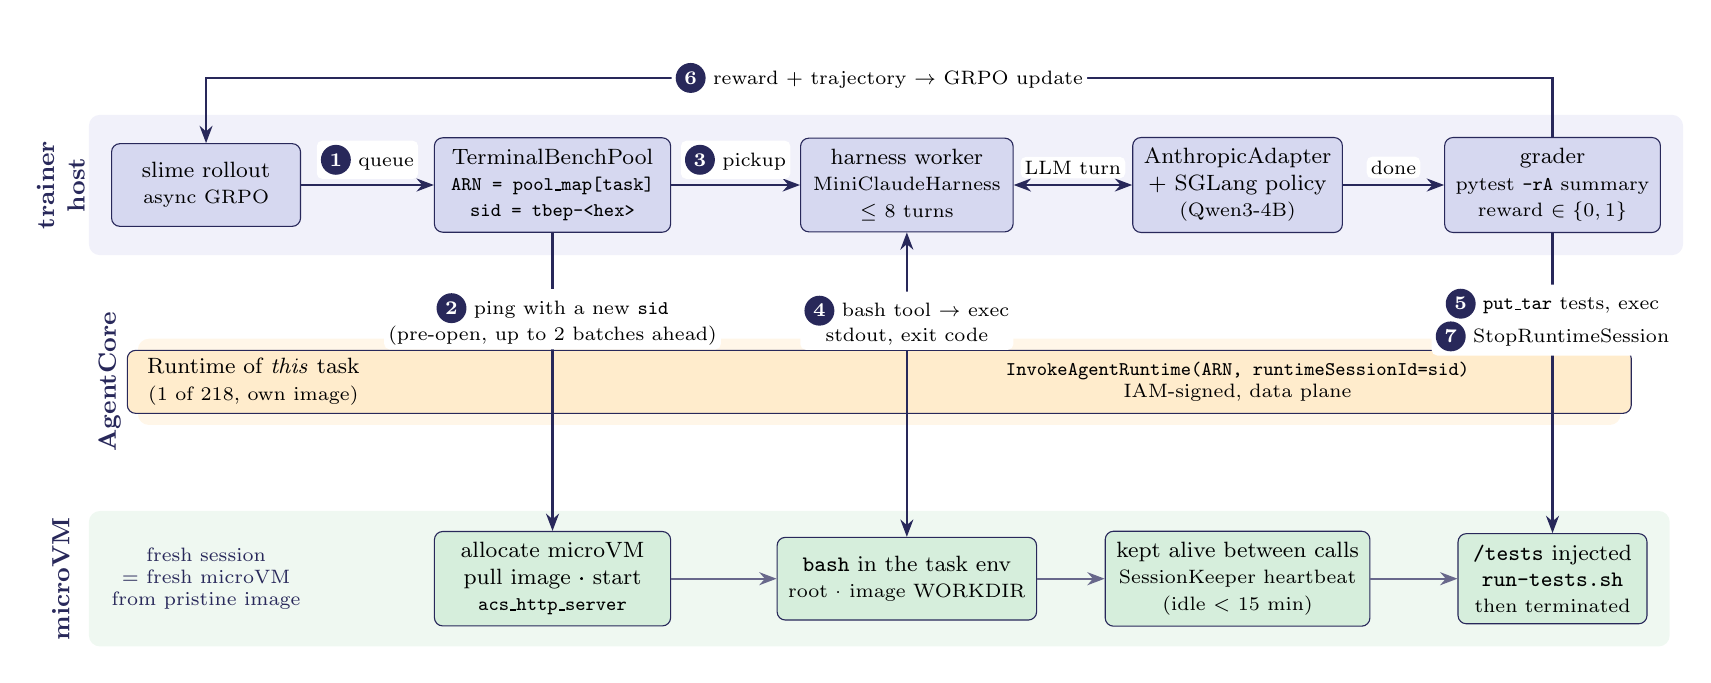
\begin{tikzpicture}[
  font=\footnotesize,
  box/.style={draw=ink, rounded corners=3pt, fill=#1, align=center, inner sep=4pt, minimum height=1.05cm},
  box/.default=host,
  arr/.style={-{Stealth[length=2.2mm]}, thick, draw=ink},
  darr/.style={{Stealth[length=2.2mm]}-{Stealth[length=2.2mm]}, thick, draw=ink},
  lab/.style={font=\scriptsize, fill=white, inner sep=1.5pt, align=center, rounded corners=2pt},
  lane/.style={font=\small\bfseries, text=ink, rotate=90, align=center},
]
% ---------------- lane 1: trainer host ----------------
\node[box, minimum width=2.4cm] (slime) at (0,0) {slime rollout\\\scriptsize async GRPO};
\node[box, minimum width=3.0cm] (pool) at (4.4,0) {TerminalBenchPool\\\scriptsize \texttt{ARN = pool\_map[task]}\\\scriptsize \texttt{sid = tbep-<hex>}};
\node[box, minimum width=2.7cm] (harness) at (8.9,0) {harness worker\\\scriptsize MiniClaudeHarness\\\scriptsize $\le$ 8 turns};
\node[box, minimum width=2.6cm] (sglang) at (13.1,0) {AnthropicAdapter\\+ SGLang policy\\\scriptsize (Qwen3-4B)};
\node[box, minimum width=2.4cm] (grader) at (17.1,0) {grader\\\scriptsize pytest \texttt{-rA} summary\\\scriptsize reward $\in\{0,1\}$};

% ---------------- lane 2: AgentCore ----------------
\node[box=ac, minimum width=19.1cm, minimum height=0.8cm] (rt) at (8.55,-2.5) {};
\node[font=\footnotesize, align=center] at (0.6,-2.5) {Runtime of \emph{this} task\\\scriptsize (1 of 218, own image)};
\node[font=\scriptsize, align=center] at (13.1,-2.5) {\texttt{InvokeAgentRuntime(ARN, runtimeSessionId=sid)}\\IAM-signed, data plane};

% ---------------- lane 3: the episode's microVM ----------------
\node[box=vm, minimum width=3.0cm] (boot) at (4.4,-5.0) {allocate microVM\\pull image · start\\\scriptsize \texttt{acs\_http\_server}};
\node[box=vm, minimum width=2.7cm] (exec) at (8.9,-5.0) {\texttt{bash} in the task env\\\scriptsize root · image WORKDIR};
\node[box=vm, minimum width=2.6cm] (idle) at (13.1,-5.0) {kept alive between calls\\\scriptsize SessionKeeper heartbeat\\\scriptsize (idle $<$ 15 min)};
\node[box=vm, minimum width=2.4cm] (tests) at (17.1,-5.0) {\texttt{/tests} injected\\\texttt{run-tests.sh}\\\scriptsize then terminated};

% ---------------- lanes (background) ----------------
\begin{scope}[on background layer]
  \node[fill=host!35, rounded corners=4pt, fit=(slime)(grader), inner xsep=8pt, inner ysep=8pt] (L1) {};
  \node[fill=ac!45, rounded corners=4pt, fit=(rt), inner xsep=-4pt, inner ysep=4pt] (L2) {};
  \node[fill=vm!40, rounded corners=4pt, fit=(slime.west |- boot)(tests), inner xsep=8pt, inner ysep=8pt] (L3) {};
  \path[use as bounding box] ($(L1.north west)+(-0.1,1.1)$) rectangle ($(L3.south east)+(0.1,-0.1)$);
\end{scope}
\node[lane] at ($(L1.west)+(-0.35,0)$) {trainer\\host};
\node[lane] at ($(L2.west)+(-0.35,0)$) {AgentCore};
\node[lane] at ($(L3.west)+(-0.35,0)$) {microVM};

% ---------------- flow ----------------
\draw[arr] (slime) -- node[lab, above=2pt] {\n{1} queue} (pool);
\draw[arr] (pool) -- node[lab, above=2pt] {\n{3} pickup} (harness);
\draw[darr] (harness) -- node[lab, above=2pt] {LLM turn} (sglang);
\draw[arr] (sglang) -- node[lab, above=2pt] {done} (grader);
\draw[arr] (grader.north) -- ++(0,0.75) -| node[lab, pos=0.25] {\n{6} reward + trajectory $\rightarrow$ GRPO update} (slime.north);

% vertical: through the Runtime to the microVM
\draw[arr] (pool.south) -- node[lab, pos=0.29] {\n{2} ping with a new \texttt{sid}\\(pre-open, up to 2 batches ahead)} (boot.north);
\draw[darr] (harness.south) -- node[lab, pos=0.29] {\n{4} bash tool $\rightarrow$ exec\\stdout, exit code} (exec.north);
\draw[arr] (grader.south) -- node[lab, pos=0.29] {\n{5} \texttt{put\_tar} tests, exec\\\n{7} StopRuntimeSession} (tests.north);

\node[font=\scriptsize, align=center, text=ink] at (0,-5.0) {fresh session\\= fresh microVM\\from pristine image};
% microVM lifetime along the bottom
\draw[arr, draw=ink!70] (boot) -- (exec);
\draw[arr, draw=ink!70] (exec) -- (idle);
\draw[arr, draw=ink!70] (idle) -- (tests);
\end{tikzpicture}
\end{document}
